% Section -- Electrical Design
% Draft 1 (22 Nov 2026). Basis: docs/assumption_register.md items X1-X8 and tools/make_sld.py.
\section{Electrical Design}
\label{sec:electrical}

\begin{figure*}[!t]
\centering
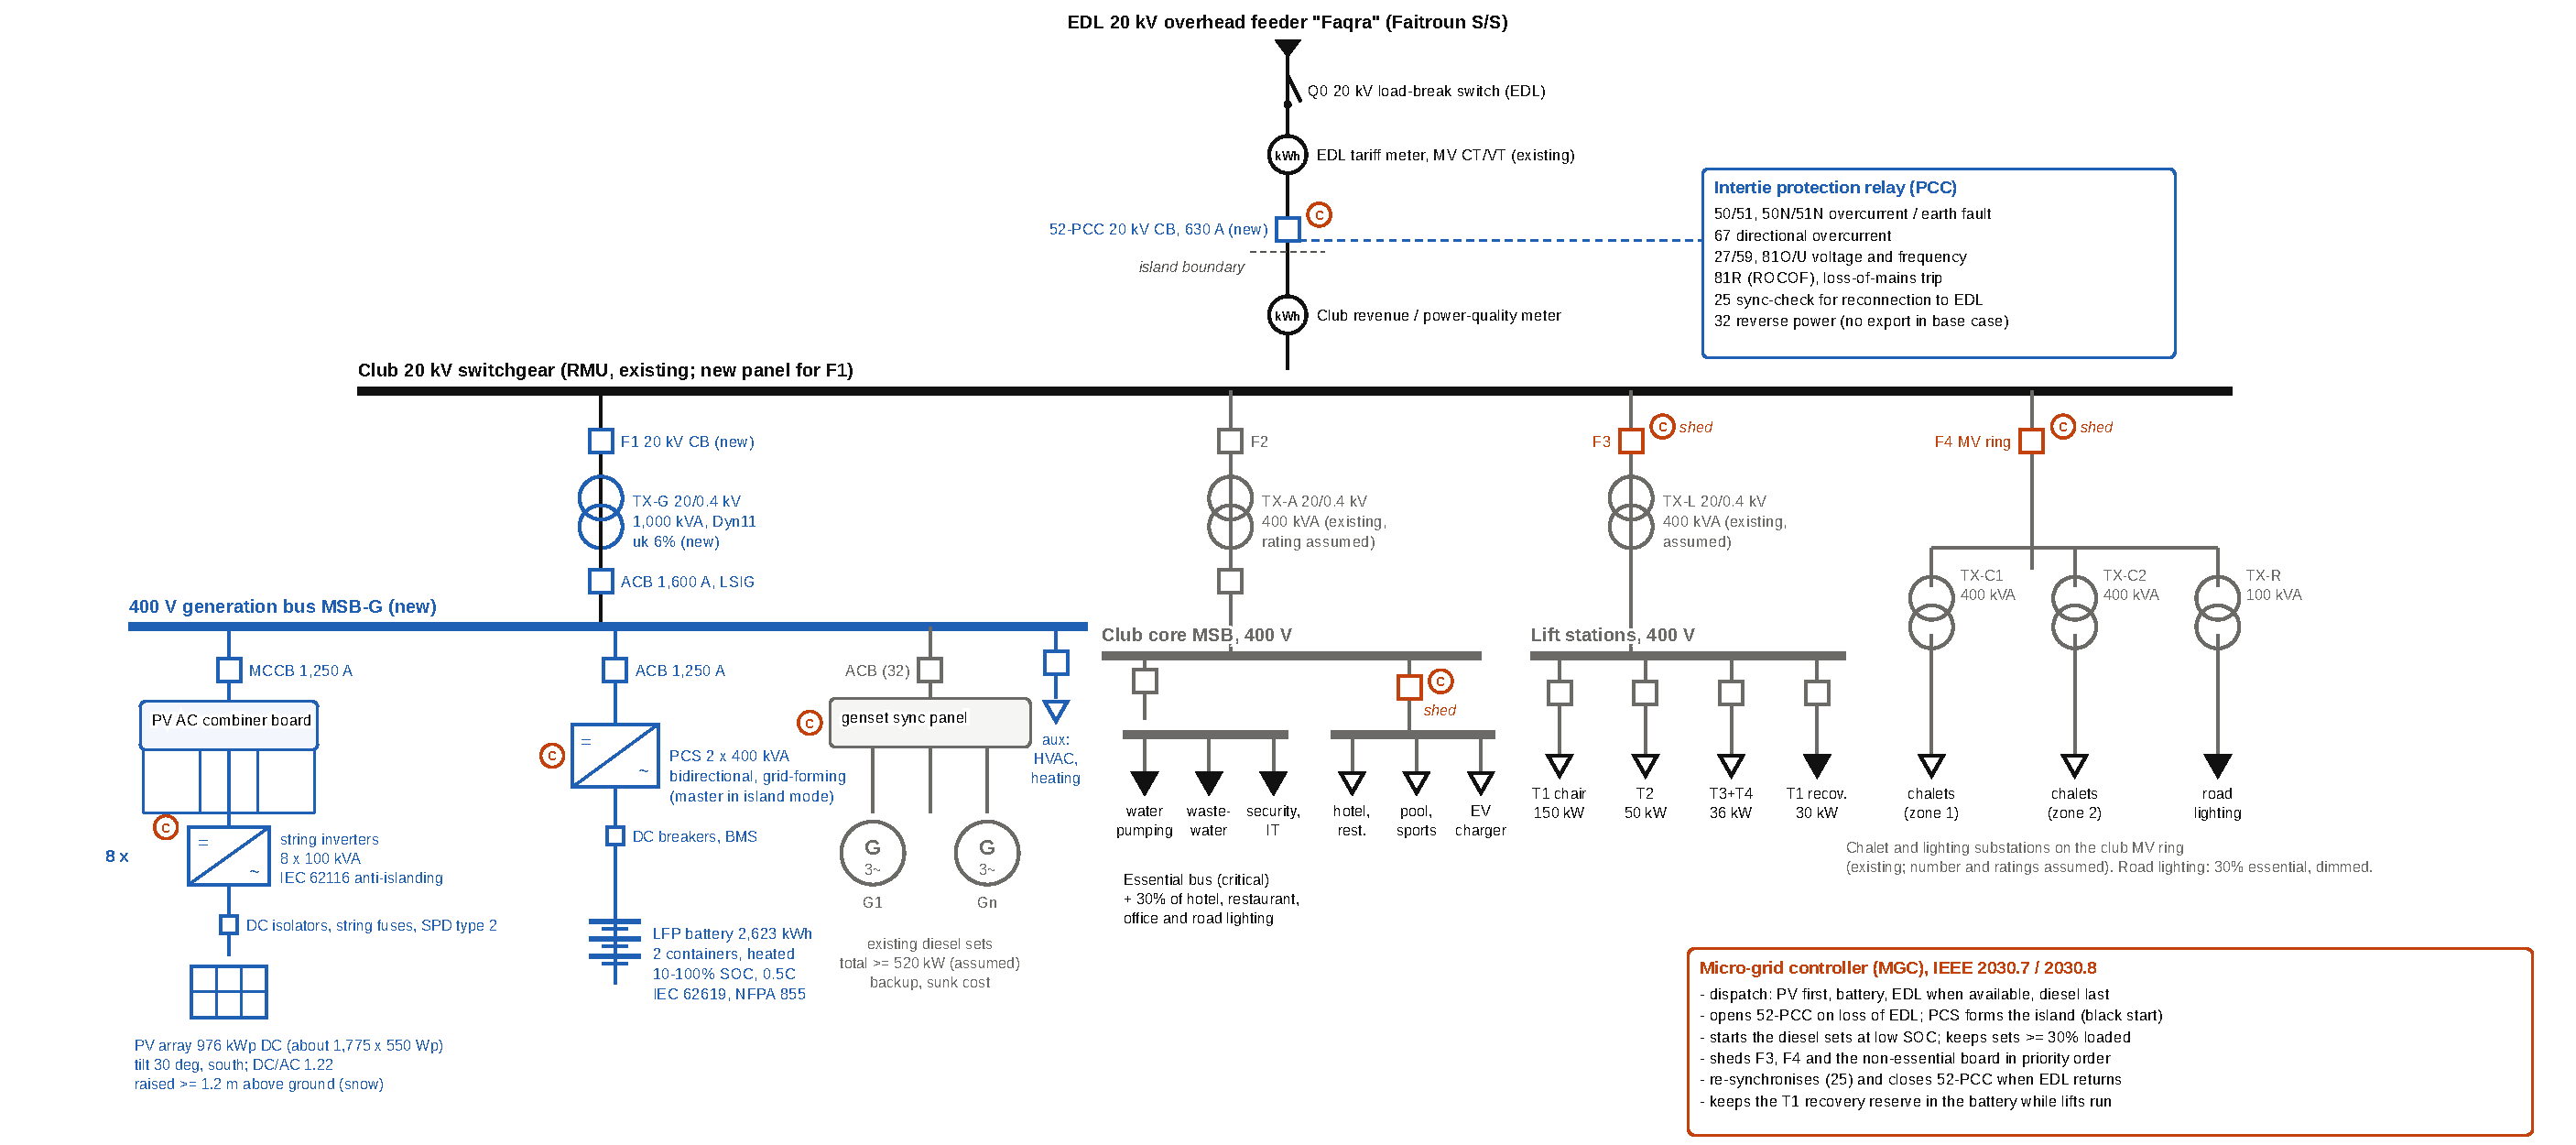
\includegraphics[width=\textwidth]{figs/sld_paper.pdf}
\caption{Single-line diagram of the base-case design. New equipment is drawn in blue and existing or
assumed equipment in grey; breakers marked C are controlled by the micro-grid controller, and those
marked ``shed'' open in priority order during long outages. Ratings of existing equipment are assumed.}
\label{fig:sld}
\end{figure*}

\subsection{Coupling Architecture and Inverter Sizing}
Fig.~\ref{fig:sld} shows the proposed layout. The PV array, the battery and the existing diesel
sets are AC-coupled on a new 400~V generation bus, which connects to the club's 20~kV switchgear
through a new feeder and a 1,000~kVA, 20/0.4~kV transformer. AC coupling lets the existing gensets
synchronize with the battery without modification and keeps each source on its own converter.
The island boundary is the club's 20~kV incomer, so the lifts, chalets and services can all be
supplied when the EDL feeder is off. In the base-case dispatch, the net flow through the transformer
peaks at 519~kW out of the generation bus and 450~kW into it, which leaves margin for the export case.

The 976~kWp array feeds eight 100~kVA string inverters, a DC/AC ratio of 1.22. The LP does not limit
the AC output of the PV; clipping at 800~kVA affects 54 hours and 3.5~MWh per year (0.3\% of the PV
energy used). The battery has two 400~kVA bidirectional converters, matching the 786~kW battery power
rating. Because the grid is off for about 16~h per day, the battery converters are grid-forming and act
as the island master, and the diesel sets follow them. The 2,623~kWh of LFP cells are housed in two
heated containers, since the battery must deliver its rated capacity through the winter.

\subsection{Protection}
A new 20~kV breaker at the point of common coupling separates the club from EDL. Its intertie relay
provides overcurrent and earth-fault protection (50/51, 50N/51N), directional overcurrent (67),
under- and over-voltage and frequency (27/59, 81O/U), rate-of-change of frequency for loss of mains
(81R), sync-check for reconnection (25), and reverse power (32), which blocks export in the base case.
These are the intertie functions required by IEEE~1547-2018. The PV inverters carry their own
anti-islanding protection (IEC~62116), so no PV is fed into a de-energized EDL line. On the 400~V
side, the transformer incomer is a 1,600~A air circuit breaker, and the PV and battery feeders each
have a 1,250~A breaker, sized for their rated currents of about 1,150~A.

\subsection{Load Partitioning}
The loads are split into an essential bus and sheddable feeders. The essential bus carries water
pumping, wastewater treatment, security and IT, 30\% of the hotel, restaurant, office and road-lighting
load, and the 30~kW recovery drive of the main chairlift (EN~13223); together these form the critical
load of Section~III, which is never shed. The lift feeder, the chalet ring and the non-essential
board each have a breaker under the control of the micro-grid controller (IEEE~2030.7/2030.8). The
controller dispatches PV first, then the battery, the grid when available and the diesel last; opens
the PCC breaker on loss of EDL and lets the battery converters form the island; starts the diesel sets
at low state of charge; and resynchronizes when EDL returns. In the base case no load is shed, so the
shedding breakers serve only as a fallback for outages longer than the design year.
